\documentclass[a4paper, 12pt]{article}

%\usepackage{cmap}
\usepackage[T2A]{fontenc}
\usepackage[utf8]{inputenc}
\usepackage[english, russian]{babel}
\usepackage{graphicx}
\usepackage[top=1in, bottom=1in, left=3.2cm, right=2.6cm]{geometry}
\graphicspath{./}
\usepackage{biblatex}
\addbibresource{lib.bib}
\linespread{1.5}

\usepackage{listings}
\usepackage{color}


\begin{document}
	
\begin{titlepage}
	\fontsize{12pt}{12pt}\selectfont
	\begin{figure}[t!]
		\centering
		
\includegraphics[scale=0.8]{bmstu}
	\end{figure}
	
	\noindent\rule{15cm}{3pt}
	\newline\newline
	\noindent 
	ФАКУЛЬТЕТ 
	\underline{«Информатика и системы управления»} \newline\newline
	
	\noindent КАФЕДРА \underline{«Программное обеспечение ЭВМ и информационные технологии»}\newline\newline\newline\newline\newline\newline
	
	\centering {\LARGE Отчет по лабораторной работе № 4}
	\vspace{3mm}
	
	\centering {\LARGE По курсу "Анализ Алгоритмов"
		\vspace{10mm}	
		
		\centering \bf Параллельное умножение матриц}
	\vspace{10mm}
	
	
	\begin{flushright}
		{\large	Студент:\\ Турсунов Жасурбек Рустамович \\ Группа: ИУ7-56Б
			\vspace{5mm}
			\\Преподователи: \\ Волкова Лилия Леонидовна \\ Строганов Юрий Владимирович}
	\end{flushright}
	
	\begin{center}
		\vfill
		Москва, \the\year
		~г.
	\end{center}
\end{titlepage}

\tableofcontents
\clearpage
\newpage

\section*{Введение}

\begin{flushleft}
	\hspace*{5mm} Целью данной лабораторной работы является изучение возможности параллельных вычислений и использование такого подхода на практике.\\ В данной лабораторной работе рассматривается классический алгоритм умножения матриц и параллельный алгоритм классического алгоритма умножения матриц. Необходимо сравнить зависимость времени работы алгоритма от числа параллельных потоков и размера матриц. Также следует провести сравнение стандартного и параллельного алгоритмов.
\end{flushleft}
\clearpage
\newpage
\section{Аналитическая часть}
\begin{flushleft}
	\hspace*{5mm} Матрицей А размера [m * n] называется прямоугольная таблица чисел, функций или алгебраических выражений, содержащая m строк и n столбцов. Числа m и n определяют размер матрицы. Если число столбцов в первой матрицы совпадает с числом строк во второй матрице, то эти матрицы можно перемножить. У произведения будет столько же строк, сколько в первой матрице и столько же столбцов, сколько во второй.
	\\ \hspace*{5mm} Пусть даны две прямоугольные матрицы A и B размеров [m * n] и [n * k] соответственно. В результате произведения матриц А и В получим матрицу C размера [m * k].\cite{mul}
	\begin{figure}[h]
		\hspace{5mm}
		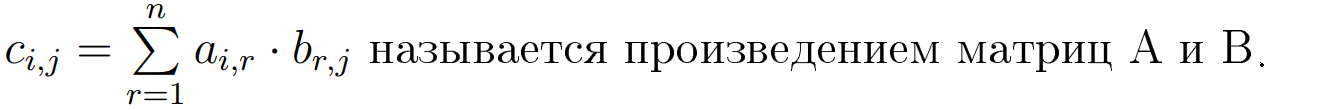
\includegraphics[scale=0.8]{formula1}
	\end{figure} 
	\subsection{Параллельный алгоритм классического умножения матриц}
	\hspace*{5mm} Чтобы улучшить алгоритм, следует распараллелить ту часть алгоритма, которая содержит 3 вложенных цикла. Вычисление результата для каждой строки не зависит от результата выполнения умножения для других строк. Поэтому можно распараллелить часть кода, где происходят эти действия. Каждый поток будет выполнять вычисления определенных строк результирующей матрицы.
	\subsection{Параллельное программирование}
	\hspace*{5mm} При использовании многопроцессорных вычислительных систем с общей памятью обычно предполагается, что имеющиеся в составе системы процессоры обладают равной производительностью, являются равноправными при доступе к общей памяти, и время доступа к памяти является одинаковым (при одновременном доступе нескольких процессоров к одному и тому же элементу памяти очередность и синхронизация доступа обеспечивается на аппаратном уровне). Многопроцессорные системы подобного типа обычно именуются симметричными мультипроцессорами (symmetric multiprocessors, SMP).
	\\ \hspace*{5mm} Перечисленному выше набору предположений удовлетворяют также активно развиваемые в последнее время многоядерные процессоры, в которых каждое ядро представляет практически независимо функциони рующее вычислительное устройство. Для общности излагаемого учебного материала для упоминания одновременно и мультипроцессоров и много ядерных процессоров для обозначения одного вычислительного устройства.
	\\ \hspace*{5mm} Обычный подход при организации вычислений для многопроцессорных вычислительных систем с общей памятью – создание новых параллельных методов на основе обычных последовательных программ, в которых или автоматически компилятором, или непосредственно программистом выделяются участки независимых друг от друга вычислений. Возможности автоматического анализа программ для порождения параллельных вычислений достаточно ограничены, и второй подход является преобладающим. При этом для разработки параллельных программ могут применяться как новые алгоритмические языки, ориентированные на параллельное программирование, так и уже имеющиеся языки, расширенные некоторым набором операторов для параллельных вычислений.
	\\ \hspace*{5mm} Широко используемый подход состоит и в применении тех или иных библиотек, обеспечивающих определенный программный интерфейс (application programming interface, API) для разработки параллельных программ. В рамках такого подхода наиболее известны Windows Thread API. Однако первый способ применим только для ОС семейства Microsoft Windows, а второй вариант API является достаточно трудоемким для использования и имеет низкоуровневый характер. \cite{paral}
	\subsection{Организация взаимодействия параллельных потоков}
	\hspace*{5mm} Потоки исполняются в общем адресном пространстве параллельной программы. Как результат, взаимодействия параллельных потоков можно организовать через использование общих данных, являющихся доступными для всех потоков. Наиболее простая ситуация состоит в использовании общих данных только для чтения.
	\clearpage
	\newpage
	В случае же, когда общие данные могут изменяться несколькими потоками, необходимы специальные усилия для организации правильного взаимодействия.
	\subsection{Вывод}
	\hspace*{5mm} Были рассмотрены алгоритмы классического умножения матриц и возможность его оптимизации с помощью распараллеливания потоков. Была рассмотрена технология параллельного программирования и организация взаимодействия параллельных потоков.
\end{flushleft}

\newpage
\section{Конструкторская часть}
\begin{flushleft}
	{\bf Требования к вводу: } На вход подаются две матрицы.
	\\ {\bf Требования к программе: }
	\begin{enumerate}
		\item корректное умножение двух матриц;
		\item при матрицах разных размеров программа не должнв аварийно завершаться. 
	\end{enumerate}
	\subsection{Разработка алгоритмов}
	В данном разделе будут рассмотрена схема алгоритма:
	\begin{enumerate}
		\item классический алгоритм умножения матриц;
	\end{enumerate}
	\clearpage
	\newpage
	\hspace*{5mm} На рисунке 1 представлена схема классического алгоритма умножения матриц.
	\begin{figure}[h!]
		\centering 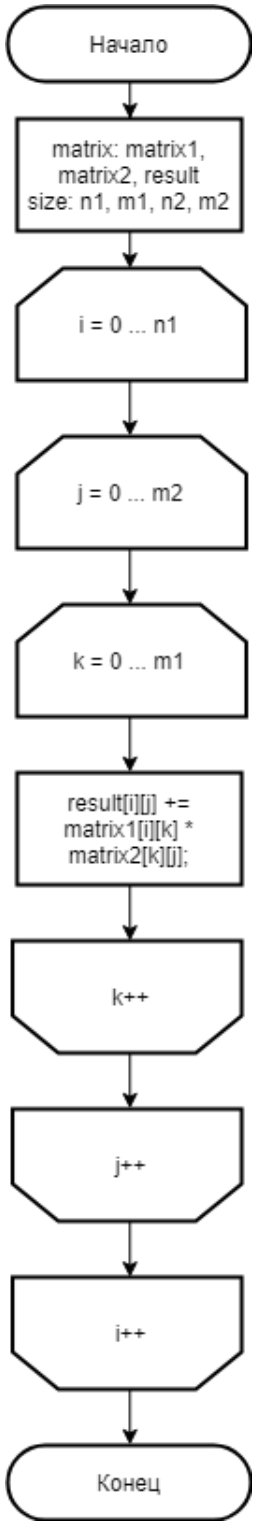
\includegraphics[scale=1.2]{classic}
		\centering \caption{Схема классического алгоритма умножения матриц}
	\end{figure}
	\clearpage
	\newpage

	\subsection{Распараллеливание программы}
	\hspace*{5mm} Распараллеливание программы должно ускорять время работы. Это достигается за счет реализации в узких участках(например в циклах с большим количеством независимых вычислений). В предложенном алгоритме данным участком будет являться тройной цикл поиска результата.
	
	\subsection{Вывод}
	\hspace*{5mm} В данном разделе были рассмотрена схема алгоритма классического умножения матриц и способ ее распараллеливания
\end{flushleft}

\newpage
\section{Технологическая часть}
\begin{flushleft}
	\hspace*{5mm} В данном разделе будут рассмотрены требования к программному обеспечению, средства реализации и представлен листинг кода.
	\subsection{Требования к программному обеспечению}
	\hspace*{5mm} Входные данные: две матрицы.
	\\ \hspace*{5mm} Выходные данные: матрица полученная в результате умножения двух матриц.
	\\ \hspace*{5mm} На рисунке 2 представлена IDEF0-диаграмма, описывающая функциональную схему умножения матриц.
	\begin{figure}[h!]
		\centering 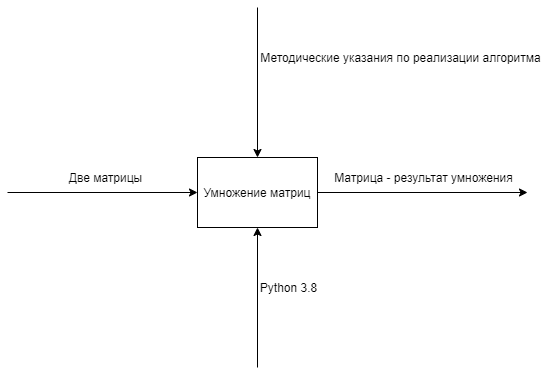
\includegraphics[scale=0.8]{диаграмма}
		\centering\caption{IDEF0-диаграмма, описывающая функциональную схему умножения матриц.}
	\end{figure}
	\clearpage
	\newpage
	\subsection{Средства реализации}
	\hspace*{5mm} В данной работе используется язык программирования Python, так как ЯП позволяет написать программу за кратчайшее время. Проект выполнен в среде разработки Visual Studio Code. Многопоточное программирование было реализовано с помощью ThreadPoolExecutor. \cite{doc} 
	\subsection{Листинг кода}
	В данном пункте представлен листинг кода, а именно:
	\begin{itemize}
		\item классический алгоритм умножения матриц;
		\item параллельная реализация классического алгоритма умножения матриц;
	\end{itemize}
	\definecolor{codegreen}{rgb}{0,0.6,0}
	\definecolor{codegray}{rgb}{0.5,0.5,0.5}
	\definecolor{codepurple}{rgb}{0.58,0,0.82}
	\definecolor{backcolour}{rgb}{0.95,0.95,0.92}

	\lstdefinestyle{mystyle}{
		backgroundcolor=\color{backcolour},   
		commentstyle=\color{codegreen},
		keywordstyle=\color{magenta},
		numberstyle=\tiny\color{codegray},
		stringstyle=\color{codepurple},
		basicstyle=\ttfamily\footnotesize,
		breakatwhitespace=false,         
		breaklines=false,                 
		captionpos=b,                    
		keepspaces=true,                 
		numbers=left,                    
		numbersep=5pt,                  
		showspaces=false,                
		showstringspaces=false,
		showtabs=false,                  
		tabsize=4
	}

	\lstset{style=mystyle}

	\hspace*{5mm} На листинге 1 представлен код классического алгоритма умножения матриц.
	\begin{lstlisting}[language=Python, caption = Классический алгоритм умножения матриц]
		def multi(A, B):
			if len(B) != len(A[0]):
				print("Different dimension of the matrics")
				return
	
			n = len(A)
			m = len(A[0])
			t = len(B[0])
	
			answer = [[0 for i in range(t)] for j in range(n)]
			for i in range(n):
				for j in range(m):
					for k in range(t):
						answer[i][k] += A[i][j] * B[j][k]
			return answer
	\end{lstlisting}
	\clearpage
	\newpage
	\hspace*{5mm} На листинге 2 представлен код распараллеленный алгоритм классического алгоритма умножения матриц .
	\begin{lstlisting}[language=Python, caption = Параллельный алгоритм умножения матриц]
		async def get_row(row, tmp):
			return [sum(starmap(mul,zip(row,column))) for column in tmp]
			
		async def multi_async(A, B):
			tmp = tuple(zip(*B))
			
			result = await asyncio.gather(*[get_row(row,tmp) for row in A])
			return results
		def async_mtr(A, B):
			if len(B) != len(A[0]):
				print("Different dimension of the matrics")
				return
		
			result = loop.run_until_complete(multi_async(A, B))
			return result
	\end{lstlisting}
	
	\subsection{Вывод}
	\hspace*{5mm} В данном разделе была представлена структура ПО и листинги кода программы. 
	
\end{flushleft}

\newpage
\section{Исследовательская часть }
\begin{flushleft}
	\hspace*{5mm} В данном разделе будет проведен эксперимент и сравнительный анализ.
	\subsection{Системные характеристики}
	Характеристики компьютера на котором проводился замер времени сортировки массива:
	\begin{enumerate}
		\item операционная система - Windows 10;
		\item процессор - Intel(R) Core(TM) i7-10510U CPU @1.80GHz 2.30GHz;
		\item оперативная память - 16 ГБ.
		\item количество ядер - 4
		\item количество логических процессов - 8
	\end{enumerate}
	\subsection{Постановка эксперимента}
	В рамках данного проекта были проведены эксперименты, описанные ниже:
	\begin{enumerate}
		\item Сравнение времени работы алгоритмов при четном и нечетном размере матрицы для разного количества потоков.
	\end{enumerate}
	\clearpage
	\newpage
	\subsection{Сравнительный анализ на основе замеров времени работы алгоритмов}
	Был проведен замер времени работы каждого из алгоритмов.
	\\ \hspace*{5mm} На рисунке 3 показаны результаты первого эксперимента, который производится для лучшего случая на квадратных матрицах размером от 100 х 100 до 1000 х 1000 с шагом 100. Количество потоков в данном эксперименте было равно 10 и 40. Ниже приведена полученная диаграмма:
	\begin{figure}[h]
		\centering 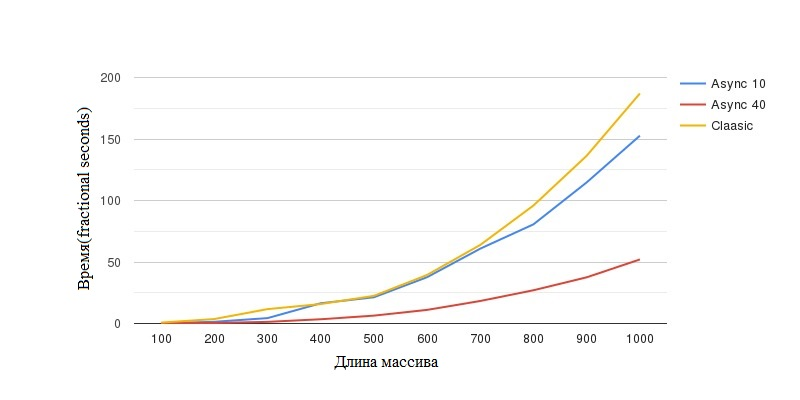
\includegraphics[scale=2]{even}
		\centering\caption{Сравнение времени работы алгоритмов при четном размере матрицы}
	\end{figure}
	
	\hspace*{5mm} На рисунке 4 показаны результаты второго эксперимента, который производится для худшего случая, когда поданы квадратные матрицы с нечетными размерами от 101 х 101 до 1001 х 1001 с шагом 100. Количество потоков в данном эксперименте было равно 10 и 40. Ниже приведена полученная диаграмма:
	\clearpage
	\newpage 
	\begin{figure}[h]
		\centering 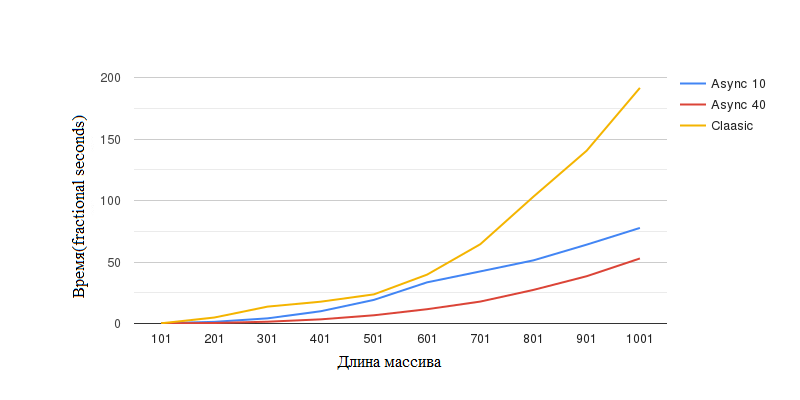
\includegraphics[scale=2]{odd}
		\centering\caption{Сравнение времени работы алгоритмов при нечетном размере матрицы}
	\end{figure}
	Третий эксперимент был проведен, для того чтобы узнать какой поток покажет лучшее время умножения матриц. Длина матрицы во время эксперимента была фиксированной и равной 400. На рисунку 5 показаны результаты этого эксперимента.
	\begin{figure}[h!]
		\centering 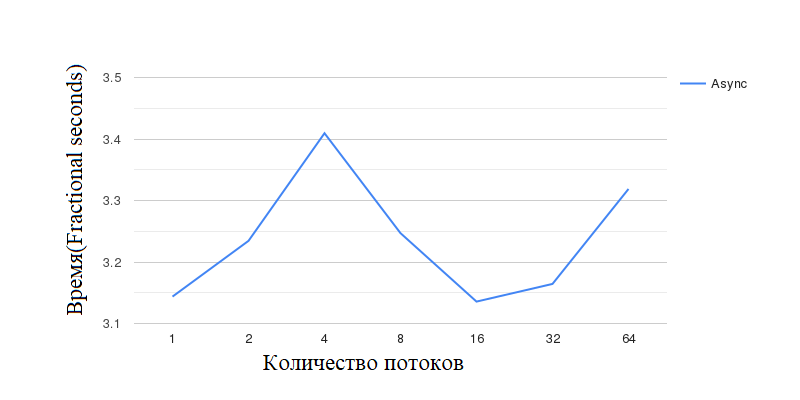
\includegraphics[scale=2]{chart}
		\centering\caption{Сравнение времени работы асинхронного алгоритмов при разном значении потоков}
	\end{figure}
	\clearpage
	\newpage
	\subsection{Тестирование программы}
	В данном разделе будут показаны результаты тестирования
	\\ \hspace*{5mm} Всего было реализовано 7 тестовых случаев:
	\begin{enumerate}
		\item некорректный размер матриц;
		\item размер матрицы равен 1;
		\item размер матрицы равен 2; 
		\item сравнение работы стандартной реализации с параллельным алгоритмом умножения на случайных значениях при четном и нечетном размерах матриц;
	\end{enumerate}
	\hspace*{5mm} На рисунке 5 показаны результаты тестирования
	\begin{figure}[h]
		\centering 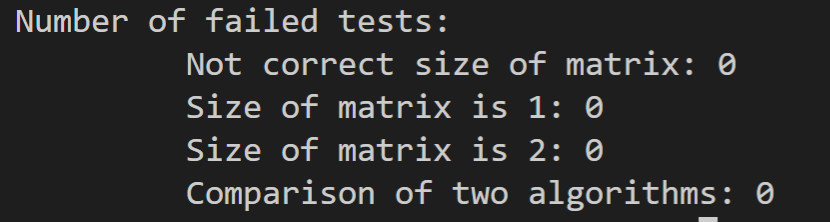
\includegraphics[scale=1.2]{tests}
		\centering\caption{Результаты тестирования}
	\end{figure}
	\subsection{Вывод}
	\hspace*{5mm} По результатам тестирования все рассматриваемые алгоритмы были реализованы верно. По проведенному анализу можно сделать вывод что классический алгоритм умножения матриц при четном и нечетном размере матриц показал худшее время по сравнению с параллельным алгоритмом. При четном размере матриц, параллельный алгоритм с количеством пулов равным 10, показал результаты близкие к классическому алгоритму. А вот параллельный алгоритм с пулов равным 40 показал лучший результат как при четном так и при нечетном размере матриц. Результаты третьего алгоритма опровдали ожидания. Лучшее время умножения было при потоке равном 16. 
\end{flushleft}

\begin{flushleft}
	\newpage
	\section*{Заключение}
	\hspace*{5mm} В ходе работы были изучены алгоритмы классического умножения матриц, стандартный и параллельный. Было сделано сравнение этих алгоритмов. В ходе сравнения было определо то, что самым быстрым оказался параллельный алгоритм при количестве пулов равным 40. В то время как классический алгоритм показал худшее время. Также можно выделить то, что дальнейшее увеличение пулов не даст значимую разницу во времени. Также был реализован программный код продукта.  
\end{flushleft}

\clearpage
\newpage

\printbibliography

\end{document}